\chapter{研究现状概述}
我们通过分析在变化网络状况下提供及时高质量的视频流所需要的性能要求,提出定制修改整个主播端的RTMP协议栈。由于现有直播架构和部署策略,非RTMP的解决方案和现在整个系统不兼容,会带来时延问题。

\section{直播系统架构}

\begin{figure}[H]% use float package if you want it here
  \centering
  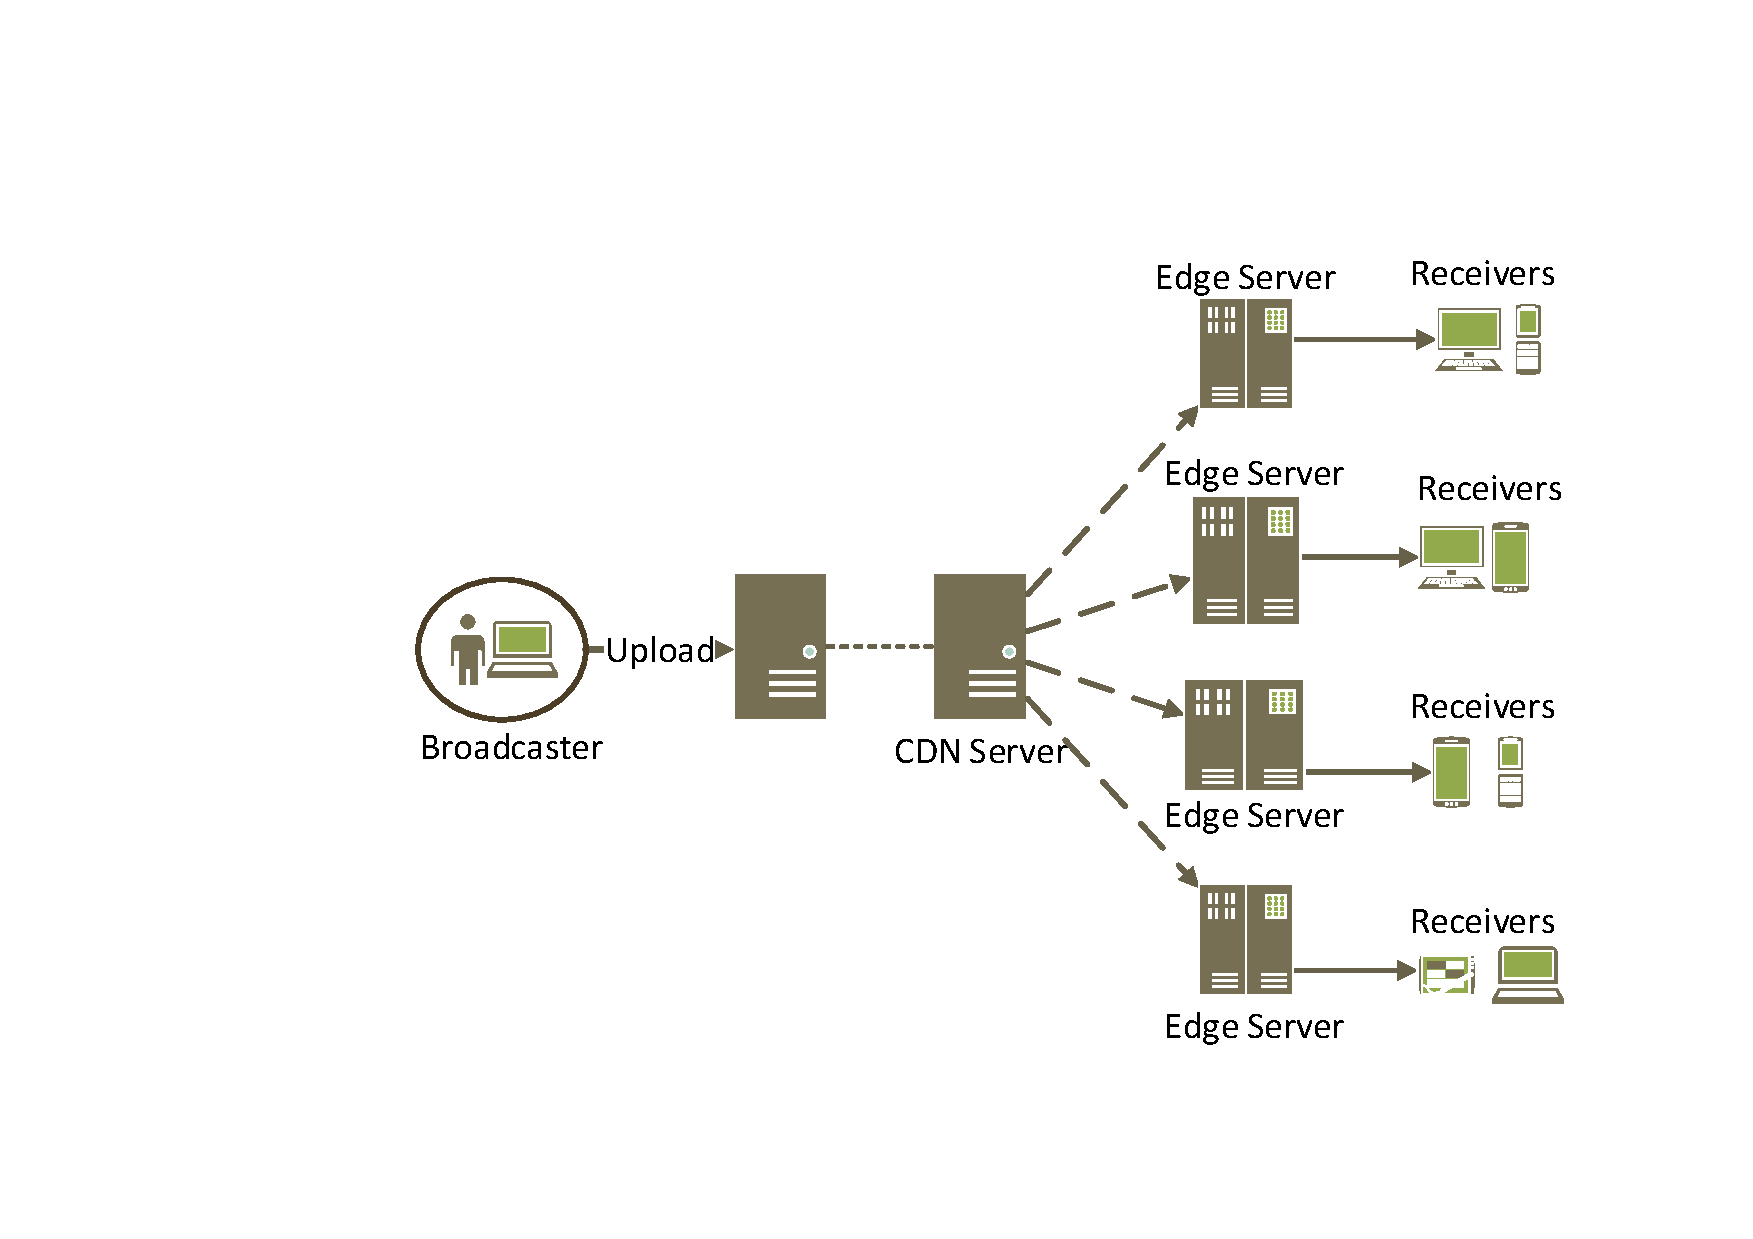
\includegraphics[width=\textwidth]{architecture}
  \caption{交互直播系统架构}
  \label{fig:architecture}
\end{figure}

图~\ref{fig:architecture}给出了个人交互直播的常用架构。直播的过程可以分为两个部分,上传和分发。开始直播时,主播端首先通过RTMP协议将直播视频流上传到源服务器;之后源服务器将视频流转发至CDN分发网络;CDN网络将视频通过传统的overlay分发协议分发至CDN边缘服务器。最后,每个用户通过HTTP流协议从最近的边缘服务器获取视频,比如,DASH等协议。

\section{交互直播}
交互直播最近繁荣发展。它从传统的直播应用演变而来,例如,ESPN的体育直播和CNN的直播。这种类型的直播都致力于将视频内容以最小的代价分发给大规模用户,同时尽量依赖于现有的CDN架构去分发。尽管个人交互直播和传统直播有这样的共同点,但个人交互直播与上述的直播有两大关键不同点,这两大不同点经常容易被忽略。
\begin{enumerate}
  \item 个人移动设备作为主播端。传统的直播,比如ESPN,使用专线连接将摄像机捕捉的高清原始视频传输到特定的内容服务器,内容服务器将原始的视频转码切分为视频块。个人交互直播不同点在于,移动用户通过无线网络上传直播的视频。无线网络状况下,主播和别人一起竞争带宽,同时由于主播的移动和环境中复杂的无线信号强度,个人交互直播可能遭受更多变的网络环境。
  \item 主播端的交互性。在传统的体育直播中,用户只是被动的观看直播。交互直播中保证端到端的时延至关重要,端到端的时延影响着主播和用户的交互体验。例如,如果用户给主播送礼,主播想要即时表示感谢。因此,直播的延迟最多为几秒,远远小于传统直播的几十秒左右的端到端时延。
\end{enumerate}

\section{性能要求}
个人交互直播和传统直播的不同点导致了主播端传输协议的如下的性能要求。
\begin{enumerate}
  \item 高码率。视频质量的指标,和视频的码率,每秒的帧率,以及分辨率有关。主播端应传输最高可用的码率到CDN服务器,这样下游的用户才能得到满意的QoE。
  \item 敏捷的码率自适应。传输协议必须足够灵活,能够快速响应无线网络中的带宽波动。
  \item 及时性。传输协议必须最小化主播端和用户之间的时延,或者限制住最大的时延。
\end{enumerate}

\section{实际部署的限制}
RTMP已经成为主流的主播端传输协议,被应用在许多商业平台上面,包括Facebook Live, Periscope,熊猫TV,斗鱼等等。RTMP协议足够灵活,有可能能够满足上述三个性能要求。比如,它在主播端提供了可调节的参数,能够调整视频质量,包括每秒的帧率,视频队列的大小,还有丢帧的策略相关参数。理论上,不同的丢帧策略可以在视频质量和及时性两者之间维持一个动态均衡。然而,我们在下个章会给出,现在商业级的RTMP实现和开源实现都存在严重的质量下降问题。

作为一个可选项,HTTP相关的直播传输协议也被广泛的研究,包括DASH,HTTP POST方式,还有两者之间的灵活切换。从RTMP切换到HTTP相关的协议虽然可能会获得更好的视频质量,但是由于每个视频块持续4-10s,不能及时的应对无线网络的波动。